\documentclass[aspectratio=1610]{beamer}

\usetheme{strath}

\usepackage[UKenglish]{babel}

\graphicspath{img/}

\title[Sample presentation]{Sample Beamer presentation}
\author[Author]{Author Name}
\institute{University of Strathclyde}
\date[2/9/22]{2nd September 2022}

\begin{document}

\frame{\titlepage}

\begin{frame}
	\frametitle{Sample frame title}
	For main/corporate theme, call \texttt{\textbackslash{}usetheme\{strath\}}
	\vspace{1cm}
	\begin{columns}
		\begin{column}{0.47\textwidth}
			\begin{enumerate}
				\item A
				\item Numbered
				\item List
			\end{enumerate}
		\end{column}
		\begin{column}{0.47\textwidth}
			\begin{itemize}
				\item Some
				\item Bullet
				\item Points
			\end{itemize}
		\end{column}
	\end{columns}
\end{frame}

\begin{frame}
	\frametitle{Engineering theme}
	\begin{columns}
		\begin{column}{0.47\textwidth}
			
\includegraphics[width=\textwidth]{eng1.png}
		\end{column}
		\begin{column}{0.47\textwidth}
			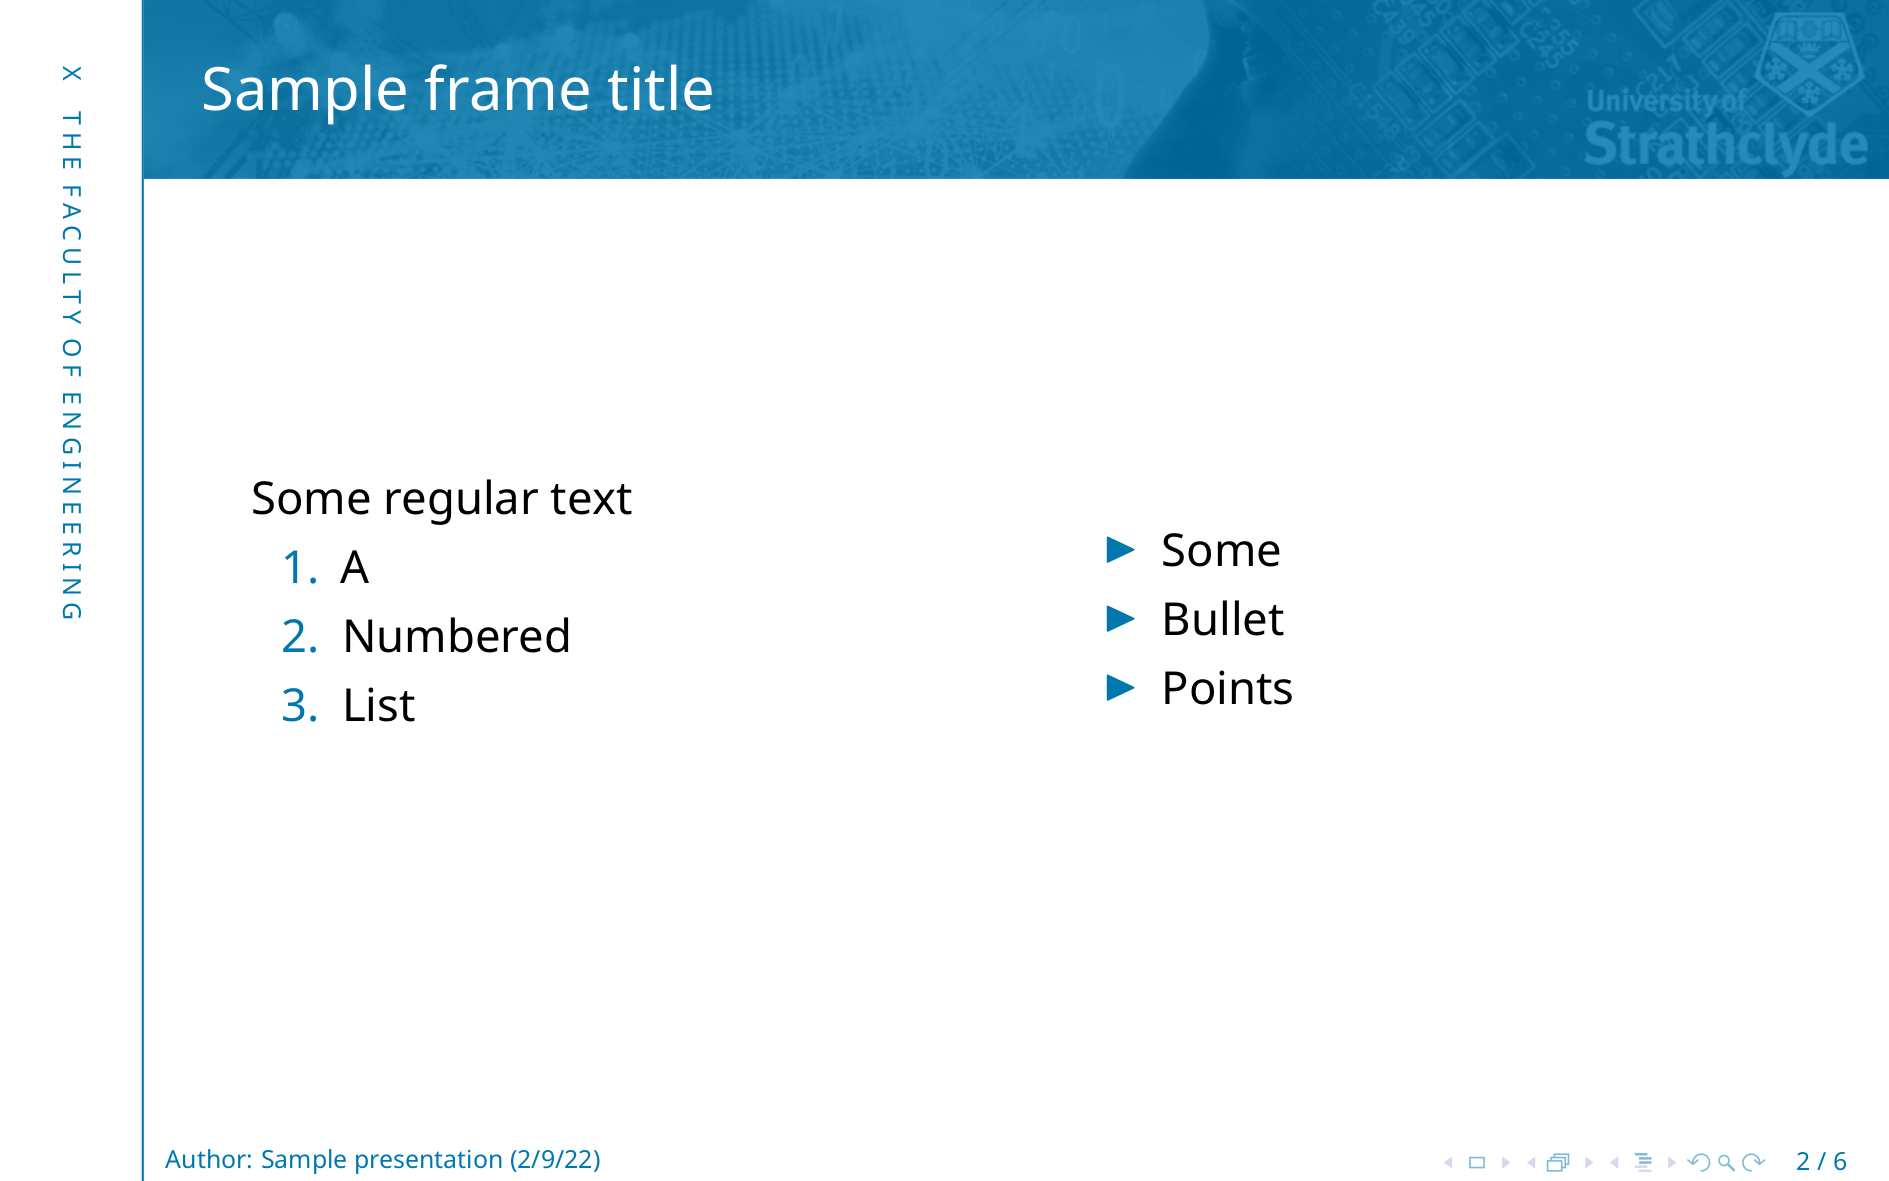
\includegraphics[width=\textwidth]{eng2.png}
		\end{column}
	\end{columns}
	\vspace{1cm}
	\centering
	\texttt{\textbackslash{}usetheme[eng]\{strath\}}
\end{frame}

\begin{frame}
	\frametitle{Science theme}
	\begin{columns}
		\begin{column}{0.47\textwidth}
			
\includegraphics[width=\textwidth]{sci1.png}
		\end{column}
		\begin{column}{0.47\textwidth}
			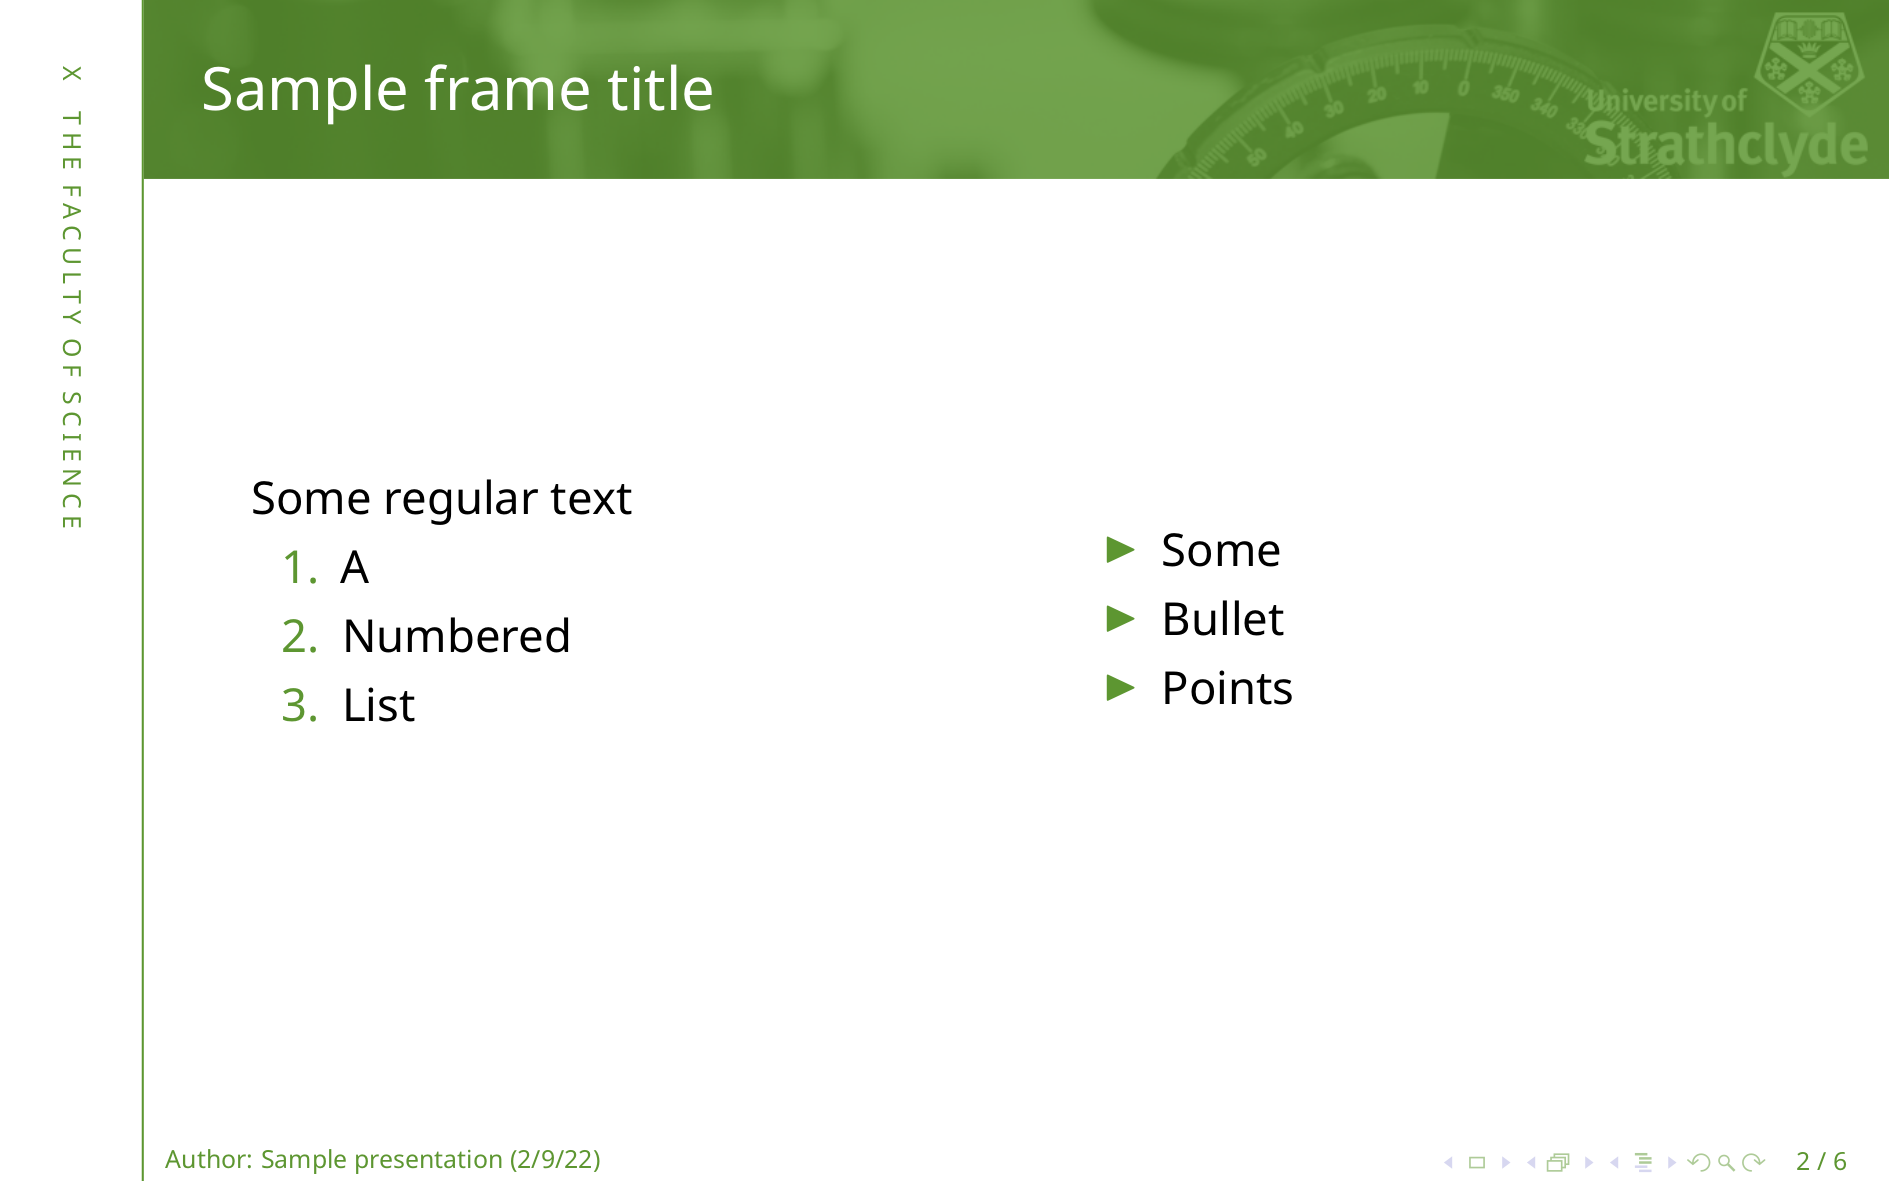
\includegraphics[width=\textwidth]{sci2.png}
		\end{column}
	\end{columns}
	\vspace{1cm}
	\centering
	\texttt{\textbackslash{}usetheme[sci]\{strath\}}
\end{frame}

\begin{frame}
	\frametitle{HaSS theme}
	\begin{columns}
		\begin{column}{0.47\textwidth}
			
\includegraphics[width=\textwidth]{hass1.png}
		\end{column}
		\begin{column}{0.47\textwidth}
			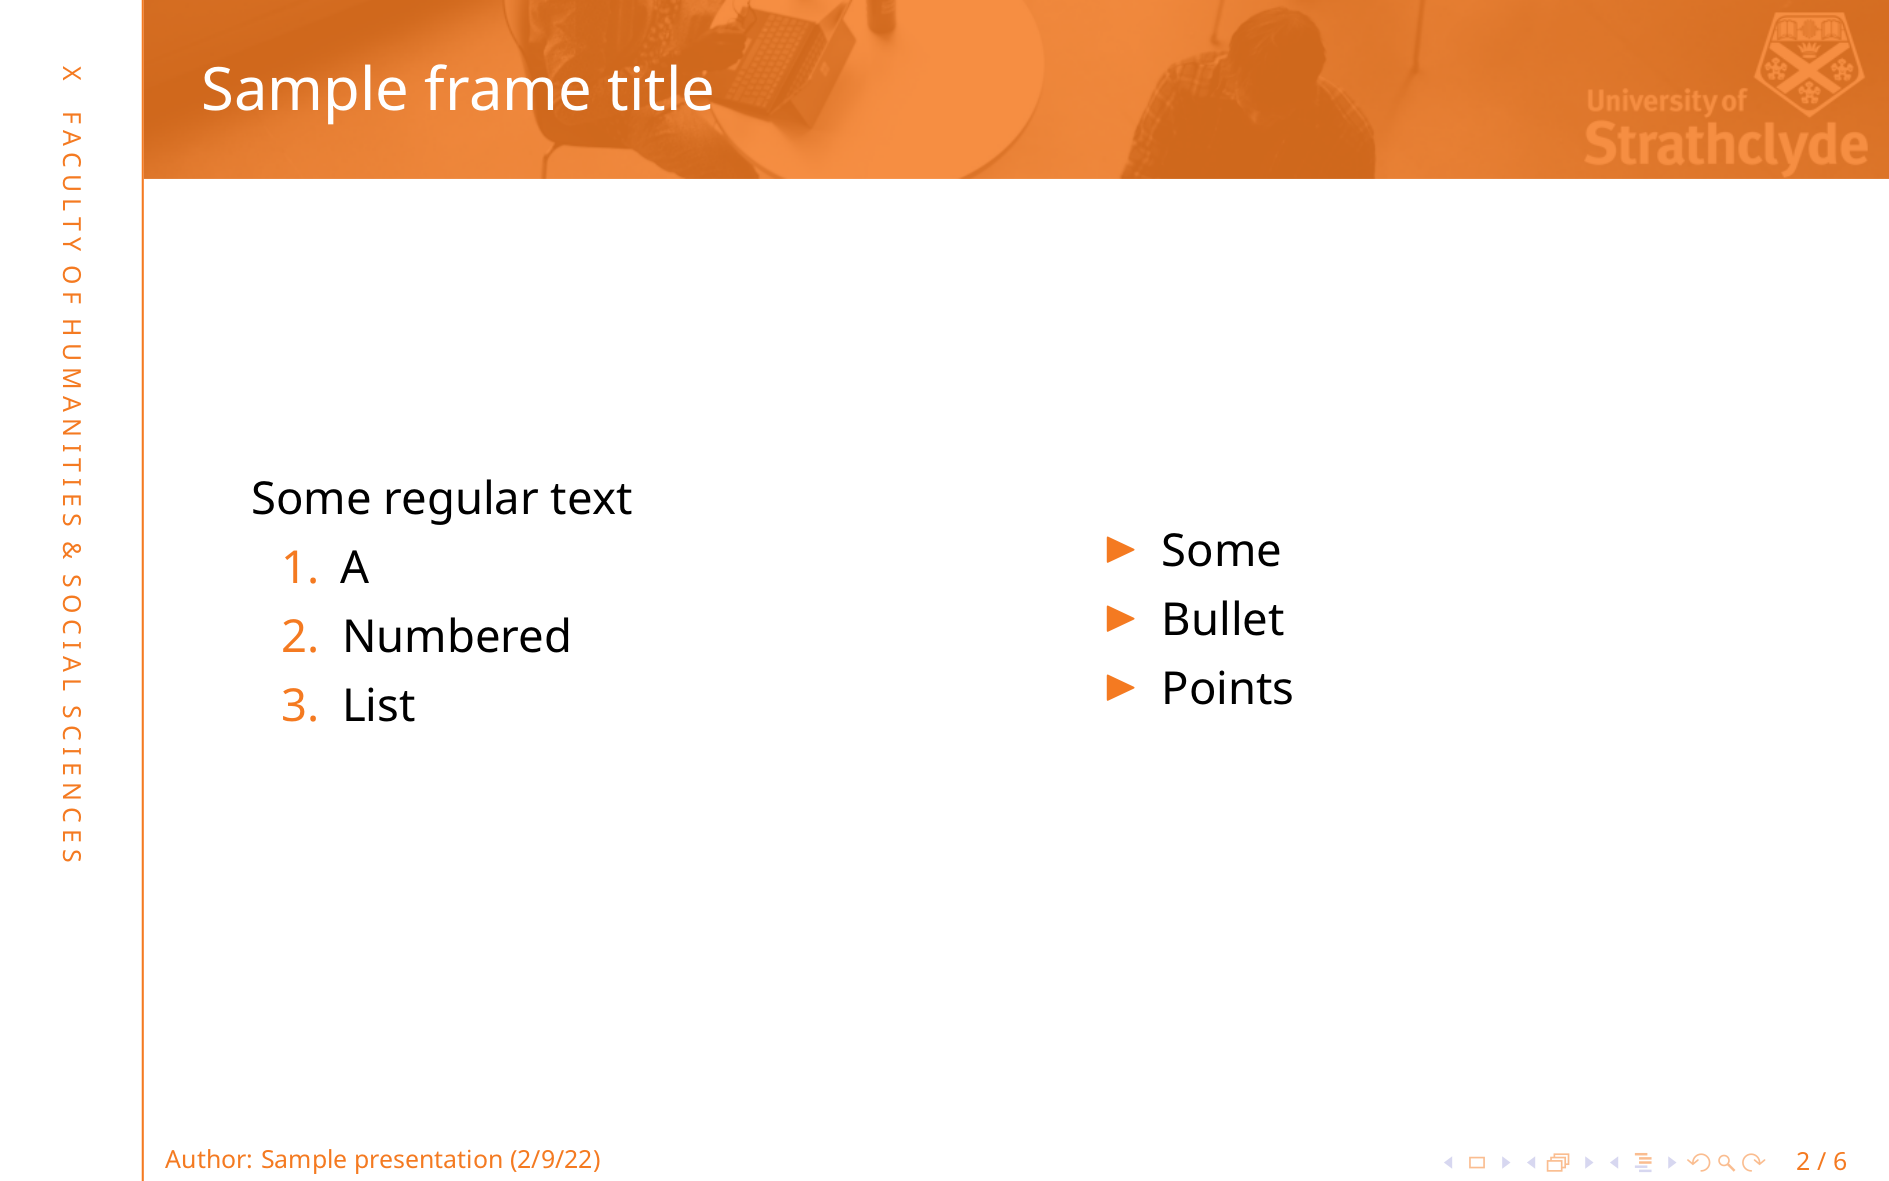
\includegraphics[width=\textwidth]{hass2.png}
		\end{column}
	\end{columns}
	\vspace{1cm}
	\centering
	\texttt{\textbackslash{}usetheme[hass]\{strath\}}
\end{frame}

\begin{frame}
	\frametitle{Business School theme}
	\begin{columns}
		\begin{column}{0.47\textwidth}
			
\includegraphics[width=\textwidth]{sbs1.png}
		\end{column}
		\begin{column}{0.47\textwidth}
			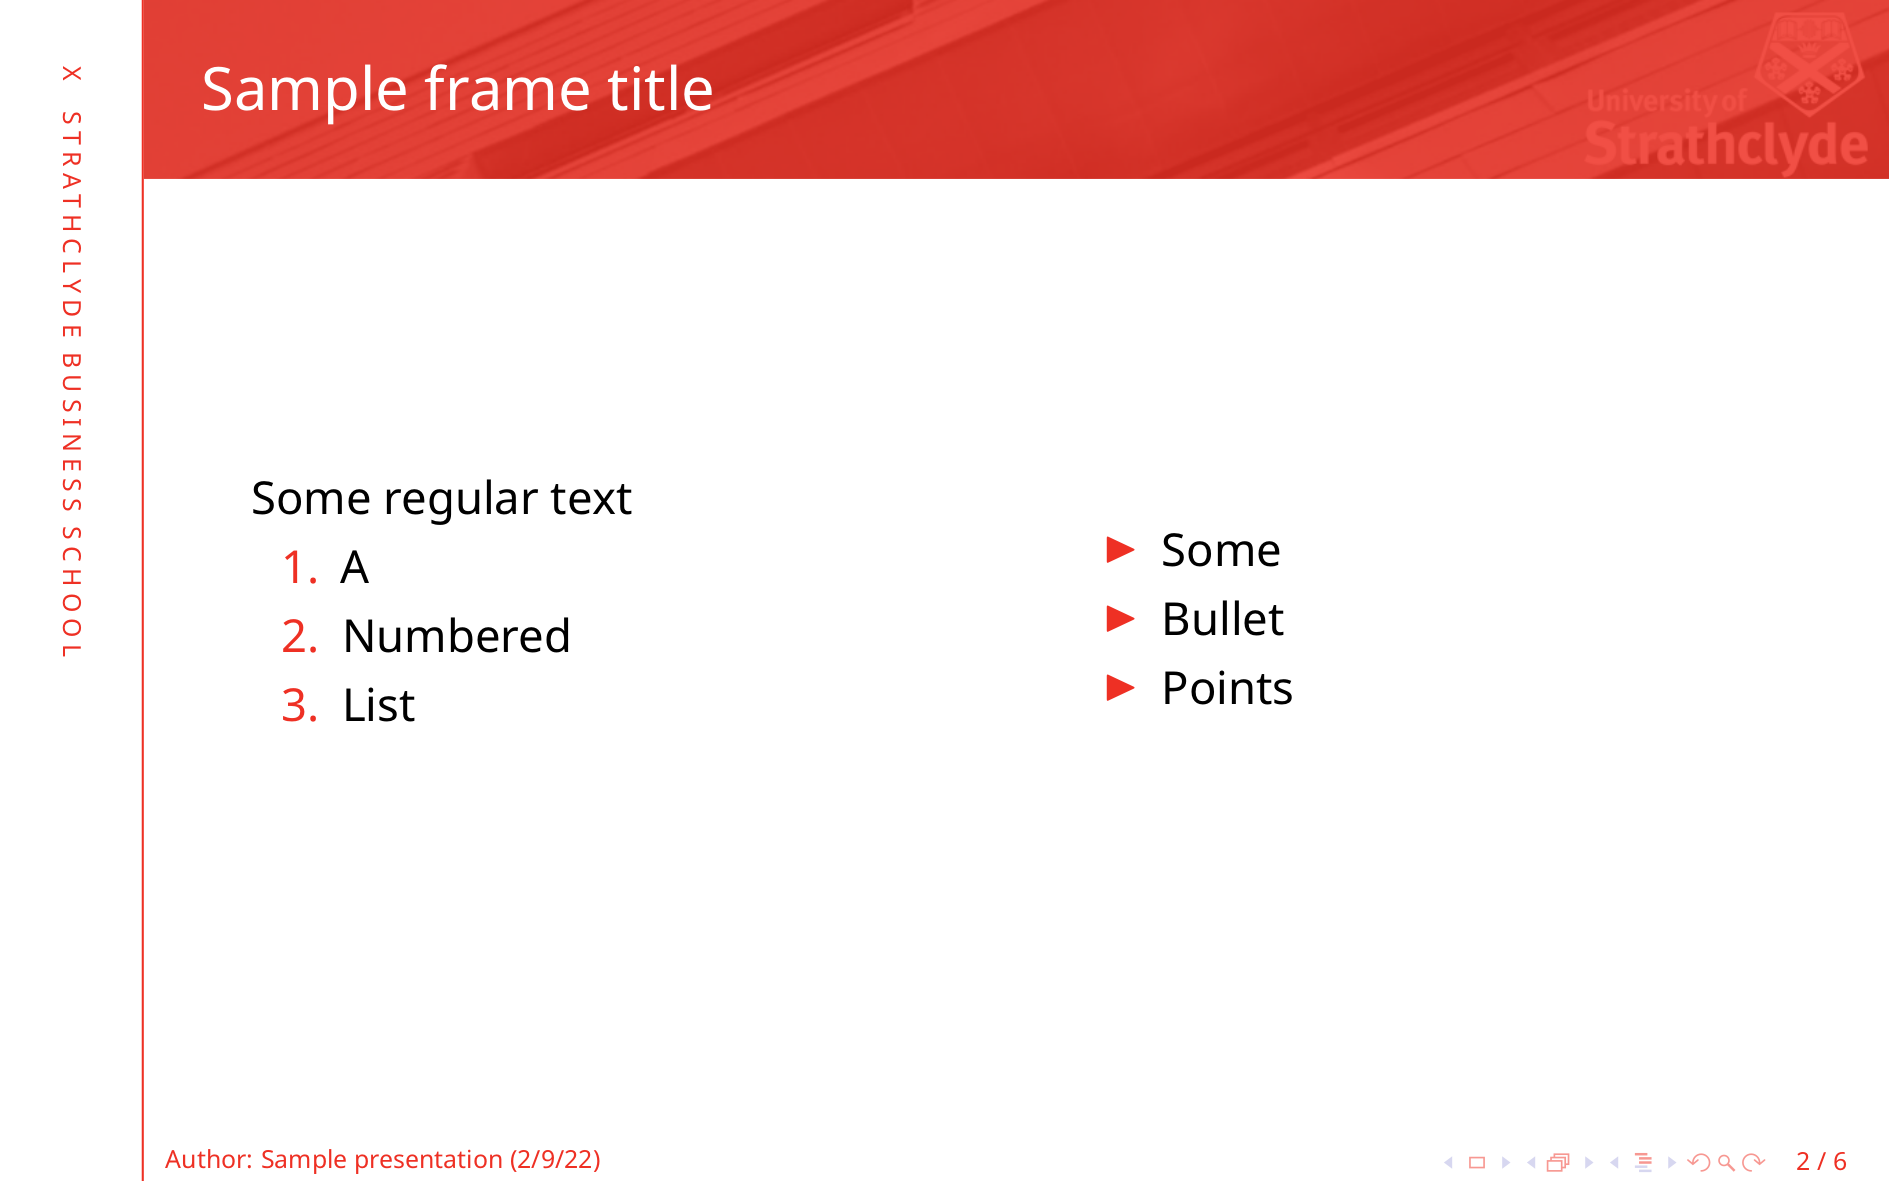
\includegraphics[width=\textwidth]{sbs2.png}
		\end{column}
	\end{columns}
	\vspace{1cm}
	\centering
	\texttt{\textbackslash{}usetheme[sbs]\{strath\}}
\end{frame}

\begin{frame}
	\frametitle{Frame title}
	\framesubtitle{Frames can have subtitles}
	\begin{block}{Block}
		Something in a regular block
	\end{block}
	\begin{exampleblock}{Example block}
		Something in an example block
	\end{exampleblock}
	\begin{alertblock}{Alert block}
		Something in an alert block
	\end{alertblock}
\end{frame}

\begin{nofootlineframe}
	\frametitle{\texttt{\textbackslash{}fillgraphics} command}
	\fillgraphics[0.47]{strath.png}
	\begin{columns}
		\begin{column}{0.47\textwidth}
			
		\end{column}
		\begin{column}{0.47\textwidth}
			\begin{block}{}\scriptsize
				First option specifies width relative to viewport (defaults to 1 for full width)
			\end{block}
			\begin{exampleblock}{Code}\tiny
				\texttt{\textbackslash{}fillgraphics[0.47]\{strath.png\}}
			\end{exampleblock}
			\begin{alertblock}{}\scriptsize
				Use \texttt{\textbackslash{}begin\{nofootlineframe\}} instead of \texttt{\textbackslash{}begin\{frame\}} to remove footline
			\end{alertblock}
		\end{column}
	\end{columns}
\end{nofootlineframe}

\begin{nofootlineframe}
	\frametitle{\texttt{\textbackslash{}fillgraphics} command}
	\fillgraphics[0.33][1]{strath.png}
	\begin{columns}
		\begin{column}{0.64\textwidth}
			\begin{block}{}\scriptsize
				Second option specifies horizontal position (defaults to 0 for left-aligned)
			\end{block}
			\begin{exampleblock}{Code}\scriptsize
				\texttt{\textbackslash{}fillgraphics[0.33][1]\{strath.png\}}
			\end{exampleblock}
		\end{column}
		\begin{column}{0.33\textwidth}
		\end{column}
	\end{columns}
\end{nofootlineframe}

\begin{nofootlineframe}
	\fillgraphics[1][0][0pt]{strath.png}
	\begin{block}{}\scriptsize
		Third option specifies top trim amount (defaults to height of frame title banner)
	\end{block}
	\begin{exampleblock}{Code}\scriptsize
		\texttt{\textbackslash{}fillgraphics[1][0][0pt]\{strath.png\}}
	\end{exampleblock}
\end{nofootlineframe}

\end{document}
